\section{Link Length Optimization}
\label{sec:link_length_optimization}
This section details the optimization of the robot's link lengths L1 and L2 to maximize jumping performance. The optimization ensures the robot can achieve sufficient jumping performance to clearly demonstrate future DRL control policies. A grid search approach using the Simscape robot model from section \ref{sec:modeling_and_simulation} systematically explores different link length configurations.



\subsection{Impact of link lengths}
Due to the lack of feedback control during the jumping maneuver, the jumping performance is determined fully by the link lengths and initial pose. By initial pose we mean the angles theta1 and theta2 of the knee and hip joints as the knee motor turns off and lets the loaded knee spring actuate the leg. Link lengths constrain the possible initial poses for any given jumping angle, while the initial pose determines spring compression through the knee angle theta2 and thus available potential spring energy. Additionally, link lengths affect the center of mass trajectory during jumps, influencing how gravitational and ground contact forces impact the robot's movement.

\subsection{Problem simplification}
First, we define the jump angle \(\theta_J\) as the angle of the velocity vector of the center of mass of the robot body at the moment the robot leaves the ground. While the robot should be able to jump both vertically and at angles sufficient to overcome obstacles, optimizing for angled jumps presents challenges. We want to directly compare the jumping performance of different link lengths, but it is not obvious how to place the initial pose of the robot to achieve a \(\theta_J\) across different link lengths. 

To simplify the optimization, only the vertical jumping performance was considered, so that different link lengths can be compared directly. Vertical jumps are achieved across link lengths by flipping the front legs such that the legs are symmetric about the vertical axis, as shown in figure \ref{fig:link_length_optimization:flipped_legs}. This flipping transforms the asymmetric leg configuration in figure \ref{fig:link_length_optimization:asymmetric_legs} where the front legs point forward into a symmetric configuration where both legs point backward. In this configuration, the movement of the legs during the jump is symmetric and the robot center of mass remains in the horizontal center of the robot, such that any horizontal component of the jump is canceled out. In practice, the robot will use the asymmetric configuration. The symmetric configuration simply provides an approximation for the jumping performance of a given link length configuration.

The metric used to evaluate the jumping performance is the maximum height reached by the center of the robot torso, minus the maximum standing height reached by the robot torso when the legs are fully extended vertically downwards and the paws are in contact with the ground. This metric will hereby be referred to as the "effective jump height".

The asymmetric leg configuration can also achieve vertical jumps by adjusting the angle between the hip-to-paw vector and vertical, as shown in figure \ref{fig:link_length_optimization:asymmetric_legs_vertical_jump}. However, finding or calculating the optimal offset for arbitrary link lengths is complex. We therefore simplify by placing paws directly beneath hips, except when $L2>L1$. While this produces less realistic jump heights, it greatly simplifies the optimization.

For $L2>L1$ configurations, placing paws directly under hips results in near-vertical legs that slip during jumps. Slipping does not occur to the same extent for asymmetric configurations with the same link lengths where the hip-to-paw angle is adjusted to give a vertical jump. In order to make the symmetric configuration a better approximation of the asymmetric case, we wish to avoid the slipping behavior. We do so by adjusting the hip-to-paw angle such that paws are slightly inward towards the body by a constant offset of 0.3 radians. This increases the vertical component of the paw force and thus the friction force (figure \ref{fig:link_length_optimization:symmetric_config_adjusted_paws}). This exact offset was chosen because experimentation showed that this makes asymmetric configuration jumps generally more vertical across a range of link lengths. This adjusted paw placement better approximates the practical asymmetric case that requires similar adjustment for vertical jumps, although the exact angle offset will vary depending on the link lengths. To handle the increased opposing horizontal forces between paws in the symmetric configuration, we double the friction coefficients from 1.0/0.8 to 2.0/1.6 (static/kinetic), which further reduces slipping.

\begin{figure}[h]
    \centering
    \begin{subfigure}[b]{0.48\textwidth}
        \centering
        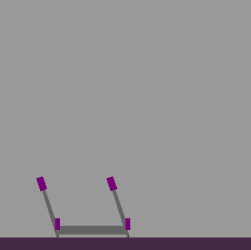
\includegraphics[width=\textwidth]{Images/link_length_optimization/unadjusted_paw_pose.png}
        \caption{Initial pose with unadjusted paws}
    \end{subfigure}
    \hfill
    \begin{subfigure}[b]{0.48\textwidth}
        \centering
        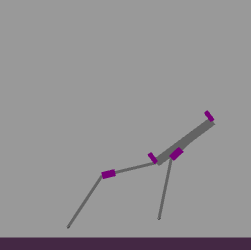
\includegraphics[width=\textwidth]{Images/link_length_optimization/unadjusted_paw_jump.png}
        \caption{Resulting angled jump}
    \end{subfigure}
    \caption{Unadjusted paw placement results in angled jump}
    \label{fig:link_length_optimization:unadjusted_jump}
\end{figure}

\begin{figure}[h]
    \centering
    \begin{subfigure}[b]{0.48\textwidth}
        \centering
        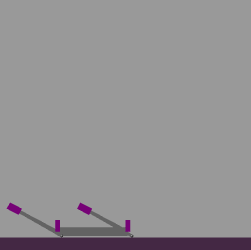
\includegraphics[width=\textwidth]{Images/link_length_optimization/adjusted_paw_pose.png}
        \caption{Initial pose with adjusted paws}
    \end{subfigure}
    \hfill
    \begin{subfigure}[b]{0.48\textwidth}
        \centering
        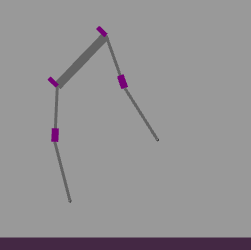
\includegraphics[width=\textwidth]{Images/link_length_optimization/adjusted_paw_jump.png}
        \caption{Resulting vertical jump}
    \end{subfigure}
    \caption{Adjusted paw placement enables vertical jump}
    \label{fig:link_length_optimization:adjusted_jump}
\end{figure}


\begin{figure}[h]
    \centering
    \begin{subfigure}[b]{0.48\textwidth}
        \centering
        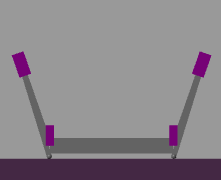
\includegraphics[width=\textwidth]{Images/link_length_optimization/symmetric_unadjusted_paws.png}
        \caption{Paws directly under hips leading to near-vertical legs}
    \end{subfigure}
    \hfill
    \begin{subfigure}[b]{0.48\textwidth}
        \centering
        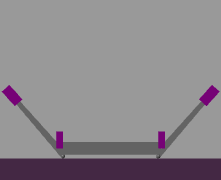
\includegraphics[width=\textwidth]{Images/link_length_optimization/symmetric_adjusted_paws.png}
        \caption{Paws translated inward to make legs more horizontal, which reduces slipping}
    \end{subfigure}
    \caption{Paw placement adjustment for $L2>L1$ configurations}
    \label{fig:link_length_optimization:symmetric_config_adjusted_paws}
\end{figure}


\begin{figure}[h]
    \centering
    \begin{subfigure}[b]{0.48\textwidth}
        \centering
        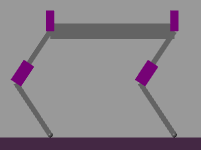
\includegraphics[width=\textwidth]{Images/link_length_optimization/asymmetric_legs.png}
        \caption{Normal asymmetric leg configuration}
        \label{fig:link_length_optimization:asymmetric_legs}
    \end{subfigure}
    \hfill
    \begin{subfigure}[b]{0.48\textwidth}
        \centering
        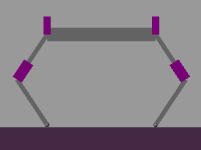
\includegraphics[width=\textwidth]{Images/link_length_optimization/symmetric_legs.png}
        \caption{Symmetric leg configuration for vertical jumping}
        \label{fig:link_length_optimization:symmetric_legs}
    \end{subfigure}
    \caption{Comparison of normal and symmetric leg configurations}
    \label{fig:link_length_optimization:flipped_legs}
\end{figure}


\subsection{Initial Pose Calculation}
For each set of link lengths, an initial pose must be calculated that satisfies several constraints:
\begin{itemize}
    \item The paws must maintain ground contact
    \item Knee angle theta2 must be maximized to store maximum spring potential energy
    \item Knees cannot penetrate the ground
    \item Both knees bend outward rather than inward
\end{itemize}

The pose calculation considers three cases based on link length ratios:

\begin{enumerate}
    \item \(L_1 = L_2\) (equal lengths)
    \item \(L_2 < L_1\) (longer lower link)
    \item \(L_1 > L_2\) (longer upper link)
\end{enumerate}

For all cases, we calculate the distance \(d\) from hip joint to paw. For cases $L1=L2$ and $L1>L2$, where paw is placed directly under hip, \(d\) is vertical from the hip. For case $L2>L1$, where paw is adjusted inwards towards the body, \(d\) is along the adjusted hip-to-paw vector. 

 \(d\) is minimized to maximize \(theta2\) and thus spring potential energy while satisfying the pose constraints. Inverse kinematics then determines \(theta1\) and \(theta2\), selecting the solution where knees bend outward. \(d\) is calculated as follows:

\begin{itemize}
    \item For \(L_1 = L_2\): \(d = \epsilon\), where \(\epsilon\) = 1mm ensures unique inverse kinematics solutions
    \item For \(L_2 > L_1\): \(d = L_2 - L_1 + \epsilon\), where \(\epsilon\) = 1mm ensures the paw position is reachable given the numerical precision of the inverse kinematics solver
    \item For \(L_1 > L_2\): \(d = \sqrt{L_1^2 - L_2^2}\), derived when \(L_2\) is horizontal (maximizing spring load) and forms a right triangle with \(L_1\) and the hip-to-paw vector
\end{itemize}

\begin{figure}[h]
    \centering
    \begin{subfigure}[b]{0.32\textwidth}
        \centering
        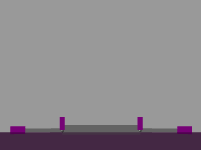
\includegraphics[width=\textwidth]{Images/link_length_optimization/equal_len_pose.png}
        \caption{Equal lengths (L1=10cm, L2=10cm)}
        \label{fig:link_length_optimization:equal_len_pose}
    \end{subfigure}
    \hfill
    \begin{subfigure}[b]{0.32\textwidth}
        \centering
        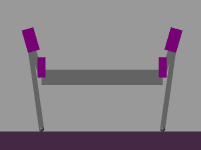
\includegraphics[width=\textwidth]{Images/link_length_optimization/longer_L2_pose.png}
        \caption{Longer L2 (L1=15cm, L2=10cm)}
        \label{fig:link_length_optimization:longer_L2_pose}
    \end{subfigure}
    \hfill
    \begin{subfigure}[b]{0.32\textwidth}
        \centering
        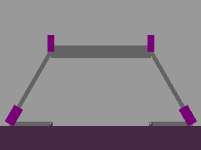
\includegraphics[width=\textwidth]{Images/link_length_optimization/longer_L1_pose.png}
        \caption{Longer L1 (L1=15cm, L2=10cm)}
        \label{fig:link_length_optimization:longer_L1_pose}
    \end{subfigure}
    \caption{Initial poses for different link length ratios}
    \label{fig:link_length_optimization:initial_poses}
\end{figure}



\subsection{Grid Search}
The grid search varies two parameters: L2/L1 ratio, and total leg length L1+L2, focusing around $L2/L1\approx1$ where preliminary tests indicated generally better performance. SimScape automatically updates the robot mass for each parameter set. Tests were run in both Earth (9.81 $m/s^2$) and Mars (3.72 $m/s^2$) gravity, with results in section \ref{sec:results:link_length_optimization}.


